% id: 142-10
% book: 100발100중 3-2 중간 · 01 3-2 중간(삼각비·삼각비의 활용·원과 직선·원주각·부록)
% section: 파이널 모의고사 3회
% figure: crop:fig-142-10.png
% answer: ②
% answer_source: 답지(빠른정답)
% variant_level: 0 (원본 전사)
% 이 파일은 build.mjs 가 items.json 에서 만든다. 고칠 때는 items.json 을 고친다.
\smash{\raisebox{1.5mm}{\dmkichul{100발100중 3-2 중간 142쪽 10번}}}
\noindent\begin{minipage}[t]{0.58\linewidth}\vspace{0pt}\raggedright 그림과 같이 반지름의 길이가 $4\mkern3mu \mathrm{cm}$인 원~$\pt{O}$에 내접하는 정팔각형의 넓이는? \mbox{[3점]}\end{minipage}\hfill\begin{minipage}[t]{0.4\linewidth}\vspace{0pt}\centering 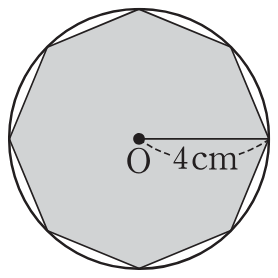
\includegraphics[width=66.5pt]{figures/fig-142-10.png}\end{minipage}\par
\begin{choicesii}{\rule[-3ex]{0pt}{8ex}$32\mkern3mu \mathrm{cm}^2$}{\rule[-3ex]{0pt}{8ex}$32\sqrt{2}\mkern3mu \mathrm{cm}^2$}{\rule[-3ex]{0pt}{8ex}$32\sqrt{3}\mkern3mu \mathrm{cm}^2$}{\rule[-3ex]{0pt}{8ex}$64\sqrt{2}\mkern3mu \mathrm{cm}^2$}{\rule[-3ex]{0pt}{8ex}$64\sqrt{3}\mkern3mu \mathrm{cm}^2$}\end{choicesii}
